\subsubsection{Magnetsensor}\label{sec: Magnetsensor}
Der Magnetsensor misst das Magnetfeld in seiner Umgebung. Der KY-024 Linearer, magnetischer Hall-Sensor\autocite{KY-024}, ist für den Dauerbetrieb geeignet und ist in einem Temperaturintervall von -150°C bis 150°C stabil. \\
\vspace{3mm}
\begin{figure}[H]
    \centering
    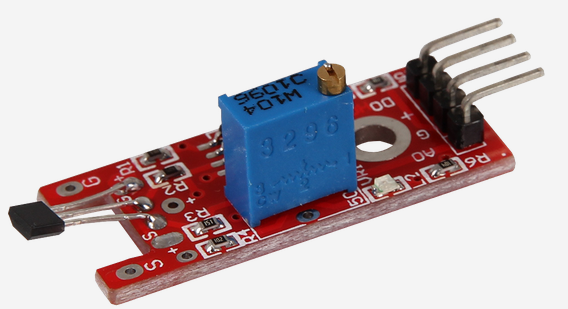
\includegraphics[scale=0.8]{image/magnetsensir.png}
    \caption{KY-024 Magnetsensor}
    \label{fig:enter-label}
\end{figure}
\vspace{3mm}
Der Sensor besitzt zwei LEDs. 
\begin{itemize}
    \item LED 1: zeigt an, ob der Sensor mit Strom versorgt wird.
    \item LED 2: zeigt an, ob der Sensor ein Magnetfeld erkannt hat.
\end{itemize}
\vspace{3mm}
Durch ein Drehpotentiometer kann die Empfindlichkeit des Sensors eingestellt werden. Über den digitalen Ausgang des Sensors wird ein Signal ausgegeben, sobald ein Magnetfeld erkannt wird.\\
\newpage
Der KY-024 ist ein analoger Sensor. Da der \raspi keinen integrierten ADC besitzt, muss einer gekauft werden, damit der Sensor über den \raspi angesteuert und gelesen werden kann. Als ADC eignet sich hierfür der 16-Bit ADC KY-053\autocite{KY-053}. \\
\vspace{2mm}
\textbf{Zusammenschaltung von \raspi, Magnetsensor und ADC}
\begin{figure}[H]
    \centering
    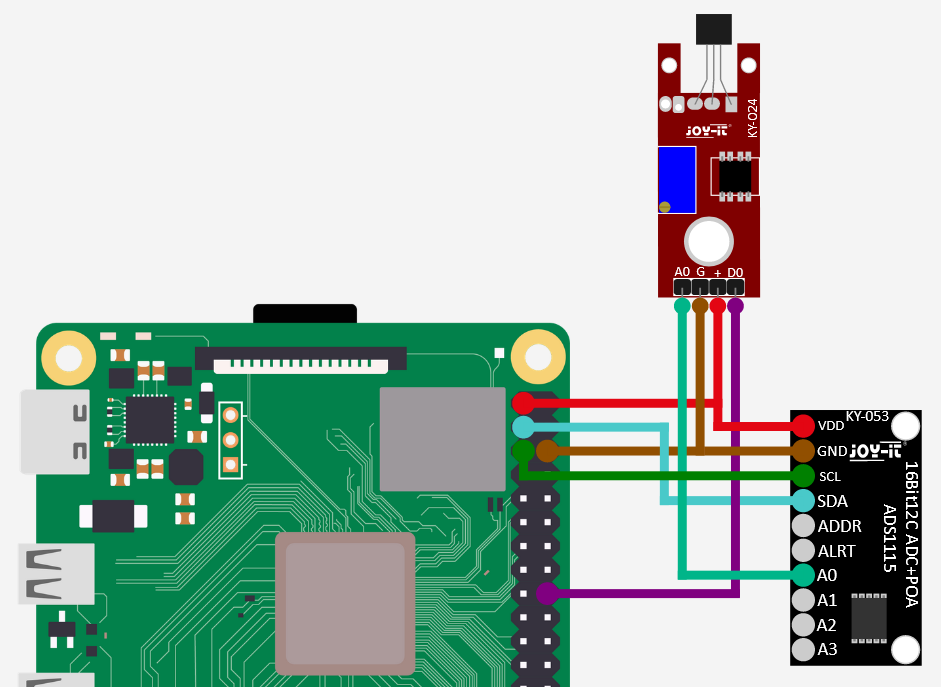
\includegraphics[scale=0.6]{image/zusammenmanet.png}
    \caption{Zusammenschaltung Magnetsensor\autocite{Zusammenschaltungmagnet}}
    \label{fig:enter-label}
\end{figure}